\documentclass[UTF8,12pt]{ctexart}
\usepackage{amsthm}
\usepackage{amsfonts,amsmath,bm}
\usepackage{graphicx}
\usepackage{xcolor}
\usepackage{geometry}

\newenvironment{myquote}
{\begin{quote}\kaishu\zihao{5}}
{\end{quote}}

\newtheorem{definition}{定义} 
\newtheorem{theorem}{定理}
\newtheorem{conjecture}{猜想}

\geometry{a4paper,scale=0.8}

\begin{document}
\title{分布式极限学习机的随机矩阵理论研究 \\ \large {————独立学习总结报告}}
\author{刘书豪 20307110229}
\date{}
\maketitle

\tableofcontents

\section{引言}
机器学习,是一门基于数据驱动,而非基于某一固定逻辑范式的算法来让机器完成某些指定任务的学科,相较于传统编程
,机器学习更加依赖算法理论的指导。具体到实现层面而言,我们希望能得到一个模型,只需要输入一个样本的特征(特
征的维度记为p)就可以得到该样本对应的结果,如预测该样本的某个指标,或是对其归类;想要得到这个模型,我们需要
大量的样本(我们记样本个数为n),通过特定的算法让机器进行学习。

传统的机器学习算法的统计分析往往都需要一个很强的假设,即n需要远远大于p[1],
一般来说,n需要超过p的200倍才行。但随着处理任务的复杂度提升,很多情况下p不仅不会远远小于n,甚至还会比n还大,
例如,在基因预测任务中每一个样本的特征数p可能是成千上万的[2],在金融领域中我们也需要构建大量的因子作为模型
的输入特征[3]。在这些情况下,使用传统的逼近理论可能无法解释机器学习模型的一些行为(一个最直观的感受是:样
本的协方差矩阵甚至可能是一个低秩矩阵),因此,我们需要一套新的理论工具。

幸运的是,随机矩阵恰好是一个有力的工具[4]。通过引入随机矩阵理论中的Stieltjes变换、Marcenko-Pastur法则、
Spiked模型等工具,在p并非远小于n的情形下,我们可以得到许多新的结论:将MUSIC算法推广到Spiked G-MUSIC算法
[5]、解释核方法在混合高斯模型分类任务中的有效性[6]、甚至还可以对某些神经网络提供理论指导,譬如计算参数初
值对MLP网络的影响[8]。

在这之中,极限学习机(Extreme Learning Machines,ELM)作为一种特殊的神经网络[9],因为其初始化权重的
随机性、单层网络的one-shot学习结构、以及较高的特征/样本维度比,十分适合使用随机矩阵进行分析。例如,近
几年来,Couillet和Louart利用随机矩阵和凝聚理论,实现了对次高斯分布分布且具有Lipschitz激活函数的ELM在训
练集和测试集上的结果预测[7],并基于此对深度学习中的二次下降现象[10][11]进行了解释[12];除此之外,他们通
过对最小二乘法中产生的核矩阵分析,为岭回归任务的梯度下降方法给出了定量的讨论[13]等。总之,利用随机矩阵理
论和凝聚理论对ELM进行理论分析是一个极具研究潜力的方向。

无独有偶,在分布式学习领域,随机矩阵也是一个不错的工具。在n并非远大于p的情况下,线性回归中产生的样本协方
差矩阵虽然不再具有传统渐近理论中的性质,但若给与一定的假设,便可基于Marcenko-Pastur法则得到其经验谱分
布的渐近表示。在分布式的学习中,尽管不会用到全部样本的协方差矩阵,但每个子样本的协方差矩阵仍然符合
Marcenko-Pastur法则,基于此我们可以得到许多结论[14]:在不同分布下分布数量对学习效率的影响,
在加入L2正则项后对于各子样本最优选取的算法设计等。

受到上述研究工作的启发,我们计划利用随机矩阵研究ELM在分布式学习下的一些渐近性质,从而加深对算法的理解
,为设计新型算法提供理论指导。

从理论研究创新角度而言,该研究课题并非是上述两个方向的简单加法。在ELM的随机矩阵研究框架下,我们并非直接
使用Marcenko-Pastur法则,而是利用凝聚理论推广到含有Lipschitz激活函数的情形,这也使得如果将分布式最小
二乘法的研究范式挪用过来,会有许多不适配的地方。实际上在[14]中,该文章更多地以经济学角度思考,花费了许
多精力研究回归系数beta产生的效应,也弱化了训练集和测试集的概念,这与ELM的研究思路是截然不同的。因此,
要做到这两者的有机融合也并非是一件易事,也仍具有一定的研究价值。同时,经过前期调研,我们也发现此前并无
其它学者从随机矩阵角度对分布式ELM进行分析,故该课题也具有一定的创新价值。

从实际应用价值角度而言,该研究课题也并非只落脚于纸上谈兵。在实际生产应用中,受限于地理位置、信息安全、
传输成本等因素,我们的数据只能储存于不同的主机或服务器。ELM作为一种one-shot的训练模型,难以在训练过
程中同时顾及不同的子数据,因此我们只能通过分别在每个子数据上进行训练,并在最后通过汇总这些训练结果并进
行加权平均来得到最终的模型参数。在这种情况下,如何确定加权平均的系数,不同子模型的随机参数是否需要一
致,正则化参数该如何选择,这些都是值得讨论的话题。

本文将首先阐述已有的相关理论,再以此为工具对分布式MLE进行理论分析。

\section{相关理论}
\subsection{极限学习机}

极限学习机是一种单层神经网络,其结构如下图所示。
\begin{figure}[htbp]
    \centering
    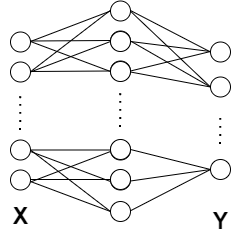
\includegraphics[width=0.5\textwidth]{ELM.png}
    \caption{极限学习机结构图}
\end{figure}

它看上去和单隐层的多层感知机(MLP)结构一致,但他们的训练方式却有着本质的不同。
MLP的训练过程是一个迭代的过程,每次迭代都会更新网络中的权重,直到网络的输出结果收敛到期望的结果。
而ELM的训练过程是一个one-shot的过程,即只需要一次迭代就可以得到网络的最终权重。
这种训练方式的好处是训练速度快,但缺点也很明显,即网络的泛化能力较差,容易出现过拟合的现象。

具体而言,在ELM中,从输入层到隐藏层的权重$W$是随机初始化的,而从隐藏层到输出层的权重$\beta$则是通过最小二乘法得到的。
即我们需要求解下面的优化问题:
\begin{equation}
    \min_{\beta} \sum_{i=1}^{n}||y_i - \sum_{j=1}^{m} \beta_j h_j(x_i)||^2,
\end{equation}
其中,$h_j(x_i)$是隐藏层第$j$个神经元的输出,即
\begin{equation}
    h_j(x_i) = \sigma(\sum_{k=1}^{p} w_{jk} x_{ik} + b_j),
\end{equation}
其中,$\sigma$是激活函数,一般为sigmoid函数或者ReLU函数。

我们可以将上述优化问题写成矩阵形式:    
\begin{equation}
    \min_{\beta} \frac{1}{N} ||Y - \beta^T \Sigma ||_F^2,
    \quad where \;\; \Sigma = \sigma(WX),
\end{equation}
其中,$X \in \mathbb{R}^{p \times N}, W \in \mathbb{R}^{n \times p}, 
\beta \in \mathbb{R}^{n \times d}, Y \in \mathbb{R}^{d \times N}$。

更一般地,我们可能还会考虑加入正则项的版本:
\begin{equation}
    \min_{\beta} \frac{1}{N} ||Y - \beta^T \Sigma ||_F^2 + \gamma ||\beta||_F^2,
\end{equation}

利用梯度求导,很容易得到最优解:
\begin{equation}
    \beta^* = \frac{1}{N} \Sigma (\frac{1}{N}\Sigma^T \Sigma + \gamma I)^{-1} Y^T.
\end{equation}

为方便起见,我们记$Q = (\frac{1}{N}\Sigma^T \Sigma + \gamma I)^{-1}$,即:
\begin{equation}
    \beta^* = \frac{1}{N} \Sigma Q Y^T.
\end{equation}

关于ELM的理论可行性,黄广华教授在其论文[9]中出了相关证明,由于和主线内容无关,这里不再赘述。

\subsection{凝聚理论}
为了对ELM进行理论分析,我们需要引入凝聚理论的相关知识:

\begin{theorem}\label{Thm0}
    如果 $\mu$ 是一个 $\mathbb{R}^d$ 上的标准高斯分布, $f$ 是一个$\mathbb{R}^d \rightarrow \mathbb{R}$ 的Lipschitz函数,且其Lipschitz常数为$\lambda_f$, 则我们有:
    \begin{equation}
        \mu(\{|f - \int fd\mu| > t\} \le Ce^{-c\frac{t^2}{\lambda_f^2}}).
    \end{equation}
\end{theorem}

上述定理告诉我们,其上的Lipschitz函数的偏离程度是可以被控制的,这对于我们后续的分析是非常有用的。

\subsection{利用凝聚理论对极限学习机进行分析}

本小节内容均摘自论文[7]。

受篇幅限制,这里仅仅罗列相关核心结论,具体证明过程请参考原论文。

在开始之前,我们先对模型加上一些假设:

\begin{itemize}
    \item[假设1 ] \textbf{随机矩阵$W$服从Sub-Gaussian分布,即存在某Lipschitz系数为
    $\lambda_\phi$的函数$\phi$,使得$W = \phi(\tilde W)$,其中$\tilde W$是一个标准高斯分布。}
\end{itemize}

显然这个假设的成立是基于凝聚理论的工具的。实际上这是一个很强的假设,例如均匀分布也是一个Sub-Gaussian分布,它的$\phi(t) = \frac{2}{\sqrt{2\pi}}\int_t^\infty e^{-x^2}dx - 1$.

\begin{itemize}
    \item[假设2 ] \textbf{激活函数$\sigma()\cdot)$是一个Lipschitz函数,且其Lipschitz常数为$\lambda_\sigma$。}
\end{itemize}

显然这也是基于凝聚理论的工具的。

\begin{itemize}
    \item[假设3 ] \textbf{当n趋于无穷时,我们对数据有一定的大小限制。}
    \begin{itemize}
        \item[\textcircled{1}] $0 < \liminf_{n \rightarrow \infty} \min{\{\frac{p}{n}, \frac{N}{n}\}} \le \limsup_{n \rightarrow \infty} \max{\{\frac{p}{n}, \frac{N}{n}\}} < \infty$。
        \item[\textcircled{2}] $\limsup_{n \rightarrow \infty} ||X||_F < \infty$
        \item[\textcircled{3}] $\limsup_{n \rightarrow \infty} ||Y||_{\infty} < \infty$
    \end{itemize}
\end{itemize}

之所以要考虑n趋向于无穷的情形,是因为我们将用到随机矩阵的工具,其相关结论的往往都是在渐近情况下成立的。

下面我们罗列相关核心定理:
\begin{theorem}
    若假设1、2、3成立,则对于矩阵$Q = (\frac{1}{N}\Sigma^T \Sigma + \gamma I)^{-1}$,我们有如下的deterministic equivalent:
    $\forall \epsilon > 0, \exists c >0 s.t. $
    \begin{equation}
        ||\mathbb EQ - \bar Q|| \le cn^{-\frac{1}{2} + \epsilon},
    \end{equation}
    其中$\bar Q = (\frac{n}{N}\frac{\Phi}{1+\delta} + \gamma I_N)^{-1}, \delta = \frac{1}{N}tr\Phi\bar Q, \Phi = \mathbb E[\sigma^T \sigma]$, $\sigma$是$\Sigma$的第一行(注意$\sigma(\cdot)$指代的是激活函数,而$\sigma$指代的是行向量, 或者它也可以被写作$\mathbb E[\sigma(w^T X)^T \sigma(w^T X)]$,其中$w$是W的某一行)。
\end{theorem}

利用上述定理,我们容易得到$\frac{1}{N} \Sigma^T \Sigma$ 的经验谱分布:

\begin{theorem}
    若假设1、2、3成立, 记$\mu_n$ 是 $\frac{1}{N} \Sigma^T \Sigma$ 的经验谱分布,则我们有如下弱收敛:
    \begin{equation}
        \mu_n \stackrel{w}{\rightarrow} \bar{\mu_n},
    \end{equation}
    其中$\bar{\mu_n}$是一个确定的分布,由它的Stietjes变换$m_{\bar{\mu_n}}$唯一决定:

    $$
    \begin{cases}
        m_{\bar{\mu_n}}(z) = \frac{1}{N}tr {(\frac{n}{N} \frac{\Phi}{1+\delta_z} - z I_N)}^{-1} \\ \delta_z = \frac{1}{N}tr \Phi {(\frac{n}{N} \frac{\Phi}{1+\delta_z} - z I_N)}^{-1} \\
    \end{cases}
    $$
\end{theorem}

上述结论也将用于对分布式ELM的分析。

最后我们可以利用上述结论对ELM在训练集和测试集上的训练结果进行预测:

\begin{theorem}
    若假设1、2、3成立,$\bar Q$是定理2中的矩阵,则我们有如下结论:$\forall \epsilon > 0$,
    \begin{equation}
        n^{\frac{1}{2}-\epsilon}(E_{train} - \bar E_{train}) \stackrel{a.s}{\longrightarrow} 0,
    \end{equation}
    其中:
    \begin{align*}
        & E_{train} = \frac{\gamma^2}{N}tr (Y^T Y Q^2), \\
        & \bar E_{train} = \frac{\gamma^2}{N}tr (Y^T Y \bar{Q} 
        \left[
            \frac{\frac{1}{n}tr\Psi \bar{Q}^2}{1 - \frac{1}{n}tr{(\Psi \bar{Q})}^2} \Psi + I_N
        \right]
        \bar{Q}
        ), \\
        & \Psi = \frac{n}{N} \frac{\Phi}{1+\delta}.
    \end{align*}
\end{theorem}

\begin{conjecture}
    若假设1、2、3成立,$\bar Q$是定理2中的矩阵,测试集上的$\hat X, \hat Y$同样也遵守假设3,则我们有如下结论:$\forall \epsilon > 0$,
    \begin{equation}
        n^{\frac{1}{2}-\epsilon}(E_{test} - \bar E_{test}) \stackrel{a.s}{\longrightarrow} 0,
    \end{equation}
    其中:
    \begin{align*}
        & E_{test} = \frac{1}{\hat N}|| \hat Y^T - \hat \Sigma^T \beta||_F^2, \\
        & \bar E_{test} = \frac{1}{\hat N}|| \hat Y^T - \Psi^T_{X \bar X} \bar Q Y^T||_F^2 + 
        \frac{
            \frac{1}{n}tr Y^T Y \bar Q \Psi \bar Q
            }{
                1 - \frac{1}{n}tr {(Y^T Y \bar Q)}^2
            }\left[
                \frac{1}{\hat N}tr \Psi_{\bar X \bar X} - \frac{1}{\hat N}tr (I_T + \gamma \bar Q)(\Psi_{X \bar X}\Psi_{\bar X X} \bar Q)
            \right].\\
        & \Psi_{AB} = \frac{n}{N} \frac{\Phi_{AB}}{1+\delta}, \Phi_{AB} = \mathbb E[\sigma(w^T A)^T \sigma(w^T B)].
    \end{align*}
\end{conjecture}

注意到这是一个猜想,并没有被严格证明,尽管它在实际数据上确实是高度符合的。

\section{分布式极限学习机}
下面我们进入到分布式极限学习机的分析。该部分结论为笔者自己推导得出,但受时间和精力限制,未推出最终结果。此处仅将目前所得结果展示出来。

\subsection{定义与假设}
和直接one-shot的极限学习机相比,分布式极限学习机是分别在多个子数据上进行训练,并在最后对这些训练结果进行加权平均得到最终的结果。具体而言,我们假设数据被分为了m个子数据集:
\begin{equation}
    X = \begin{bmatrix}
        X_1 \\ X_2 \\ \vdots \\ X_m
    \end{bmatrix},
    Y = \begin{bmatrix}
        Y_1 \\ Y_2 \\ \vdots \\ Y_m
    \end{bmatrix},
\end{equation},

目前我们只考察了不加正则项的情形。而且需要注意的是,在上述对ELM的分析中,结论中用到了$Y$的值,这在训练集上当然是可行的,但在测试集上这样做显然有些不太合理,同时,原先的结论在测试集上也并没有被严格证明。所以,我们想加入一个新的假设条件,看是否能避开上述缺陷:

\begin{itemize}
    \item[假设4 ] \textbf{我们假设对于每一个$W$,均存在一个$\beta$使得数据服从如下关系式:
    \begin{equation}
        Y = \beta^T \sigma(WX) + u,
    \end{equation}

\end{document}